\textcolor{lila}{Här presenteras huvuddragen av varje problem samt den tillhörande informationen. Notera att allt runtomkring själva problemet enbart är förslag, och att varje lärare kan anpassa genomförandet efter hur hen tror att det blir bäst i en specifik klass. Problemen i avsnitt \ref{sec:Fermi} till och med \ref{sec:Sortera} är allmänna problem som inte kräver några speciella förkunskaper från läraren, förutom det som skickas med som kompletterande information. Övriga problem baseras på programmering, och det är då lättare för läraren att hjälpa till med koden om denne kan programmera. Notera dock att det är problemlösningen som står i centrum, och inte kodens specifika syntax. Lärarna får även själva välja vilket programmeringsspråk som ska användas, men som vägledning skickas ett lösningsförslag skrivet i Java. Alla problemen finns även i sin fullständiga form i appendix~\ref{appendix:Problem}.}

\subsubsection{Fermiproblem}
    \label{sec:Fermi}
 
    \textcolor{lila}{Som inledning presenteras vad ett \textsl{fermiproblem} är. Det innebär att man, i fall där ett specifikt värde är svårt alternativt omöjligt att mäta, bryter ner problemet i många små delar och uppskattar varje del för sig. På så sätt kan man uppskatta lösningen på frågor som vid första anblick kan verka omöjliga. För att illustrera detta visas även ett exempel på ett fermiproblem, samt exempel på hur man kan dela upp det i minde delar.}

    \textcolor{lila}{Eleverna får en lista med olika fermiproblem att välja mellan, och ska arbeta i grupper om 2. Först ska de gissa på svaret, och sedan beräkna det genom att dela upp i delar som man kan uppskatta. Därefter får de i mindre grupper presentera och diskutera sitt arbete. Slutligen diskuteras i helklass om resultaten kändes rimliga, hur genomförandet gick, ifall lösningsmetoden är användbar samt varför den fungerar så bra som den gör. För den sista frågan ger vi även lärararen svaret, det vill säga att det fungerar eftersom man ibland överskattar och ibland underskattar de mindre delarna, vilket gör att det slutgiltiga resultatet ofta blir en mycket bra uppskattning.}
    
    \textcolor{lila}{Målet med detta problem är att eleverna ska få träna på att göra uppskattningar, samt att bryta ner ett problem i mindre delar.}
    
    

\subsubsection{Flygplan}
    \label{sec:Flygplan}
    
    \textcolor{lila}{En Sverigekarta med utmarkerade flygplatser och flygrutter presenteras för klassen, se figur~\ref{fig:Flygplan}. Detta görs bitvis, med plats för en kort diskussion om vad frågeställningen skulle kunna vara, givet den dittills givna informationen. Med all information given får eleverna i grupper om två arbeta med en specifik sträcka, Visby-Karlstad. På vilka olika sätt kan man ta sig mellan dessa två städer? Vilken sträcka är bäst och vilka faktorer påverkar detta? Därefter specificeras uppgiften ytterligare, genom att de får reda på hur mycket det kostar att åka mellan två olika direkta flygsträckor. De ska nu hitta den \textsl{billigaste} vägen mellan Karlstad och Visby, samt vilken väg som blir billigast om man ska från Karlstad till Stockholm, men sträckan Stockholm-Göteborg är fullbokad. Den avslutande helklassdiskussionen tar bland annat upp vilka faktorer som påverkar bränslekostnaden, vilka faktorer som påverkar biljettpris för en specifik sträcka och ifall det är det totala avståndet eller antalet mellanlandningar som avgör priset för en resa.}
    
    \textcolor{lila}{Under punkten ''Ytterligare information'' diskuteras tankar bakom uppgift och diskussion. Eleverna får själva upptäcka att priset beror på sträckan, men att det också tillkommer ett fast pris för start och landning, vilket speciellt visar sig i att det för sträckan Karlstad-Göteborg blir billigare att flyga en längre sträcka, men med färre mellanlandningar. De får också själva reflektera över ytterligare faktorer som skulle kunna påverka priset, till exempel löner och vinstmarginal.}
    
    \textcolor{lila}{Detta  problem syftar till att träna eleverna på ett undersökande arbetssätt där inte alla påverkande faktorer är givna, utan måste resoneras fram av eleverna. Den leder också fram till ett ekvationssystem, vilket ger ett exempel på när dessa är användbara.}
    
    
    
\subsubsection{Fritt fall}
    \label{sec:FrittFall}
    
    \textcolor{lila}{Som en introduktion till problemet diskuterar man tillsammans i klassen vad en derivata är och hur man kan beräkna den. Därefter presenteras en bild av en fallande boll, med utmarkerade fallsträckor för olika tider, se figur~\ref{fig:FrittFall}. Frågan är nu vad man utifrån detta kan komma fram till om bollens hastighet och acceleration, vilket klassen får arbeta med i grupper om två. Tanken är att man ska konstruera en graf över sträcka som en funktion av tid, och utifrån denna använda en linjal för att rita tangenter längs med grafen och därmed skapa en graf över hastighet som en funktion av tiden. Därefter kan samma procedur genomföras för att rita accelerationen som funktion av tiden. Denna bör, med avvikningar på grund av felkällor, bli konstant och ungefär lika med tyngdaccelerationen, det vill säga ungefär~10. Avslutningsvis diskuteras denna metod med avseende på resultat och noggrannhet.}
    
    \textcolor{lila}{Tanken med problemet är att eleverna ska få använda derivata utifrån en verklig situation istället för utifrån en färdig formel, samt få en djupare förståelse för vad derivata egentligen är.} 
        
\begin{figure}
    %\centering
    \hspace{0.4cm}
    \begin{subfigure}[b]{0.45\textwidth}
        \centering
        %\hspace{-40pt}
        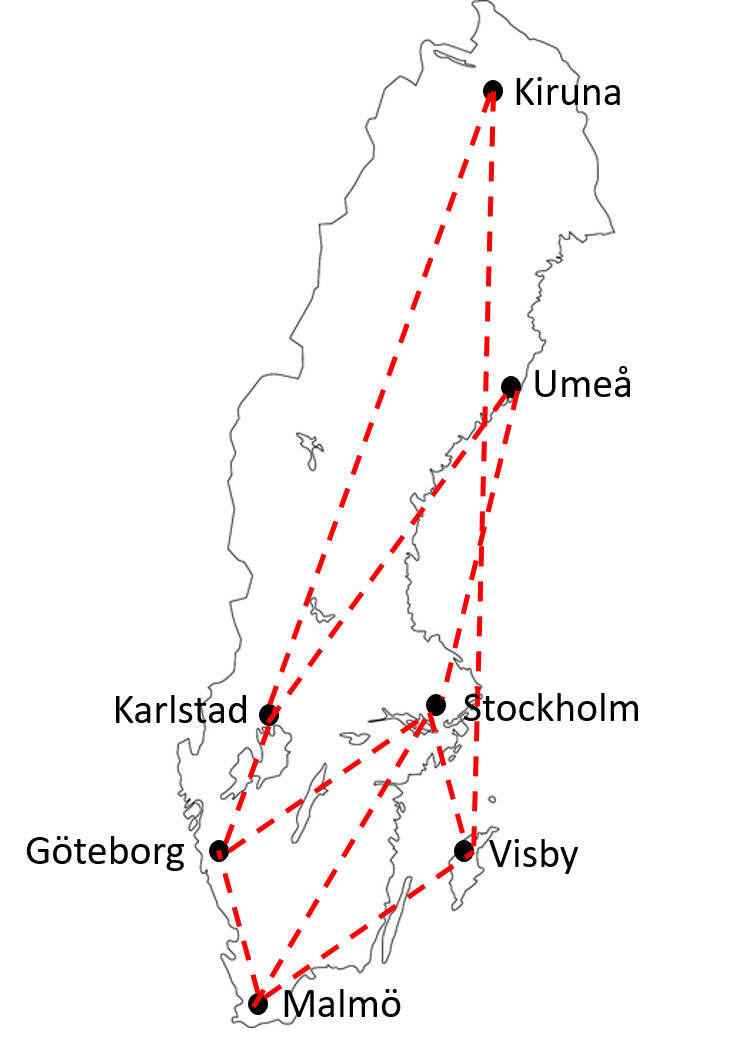
\includegraphics[width=0.9\textwidth]{Figures/Flygplan_rapport.png}
        \caption{\textsl{Sverigekarta med utmarkerade flygplatser och rutter. Bilden är baserad på \cite{SverigeKarta}}}
        \label{fig:Flygplan}
    \end{subfigure}
    \hfill
    \begin{subfigure}[b]{0.45\textwidth}
        \centering
        %\hspace{-40pt}
        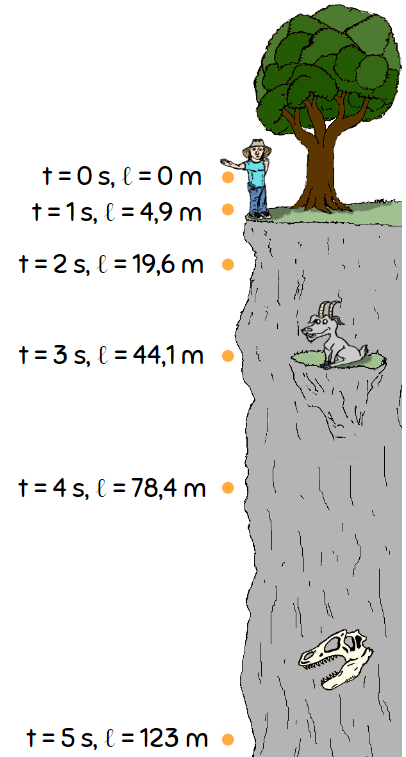
\includegraphics[width=0.7\textwidth]{Figures/FrittFall.PNG}
        \caption{\textsl{Fallande boll med angivna fallsträckor för varje sekund.}}
        \label{fig:FrittFall}
    \end{subfigure}
    \hspace{0.4cm}
    \caption{Figurer tillhörande två av problemen, ''Flygplan'' till vänster och ''Fritt fall'' till höger.}
    \label{fig:three graphs}
\end{figure}
    
    
    
\subsubsection{Försvåring av en ekvation}
    \label{sec:ekvation}

    \textcolor{lila}{Inledningsvis diskuteras begreppet ekvation, samt hur man löser en ekvation, i helklass. Det viktiga här är att komma fram till att så länge man gör samma sak på båda sidorna om likhetstecknet, och använder prioriteringsreglerna rätt, så får man göra vad som helst. Eleverna får därför två och två arbeta med att ''försvåra'' ekvationen x=2, genom att i flera steg göra en bestämd operation i både vänster- och högerledet. Följande enkla exempel på hur man kan börja presenteras för eleverna som tips på hur man kan börja}
    
        \begin{equation*}
            x=2
        \end{equation*}
        \begin{equation*}
            2x=4 \quad (\cdot2=\cdot2)
        \end{equation*}
        \begin{equation*}
            2x+5=7+2 \quad (+5=+3+2)
        \end{equation*}
    
    \noindent\textcolor{lila}{Varje steg ska även skrivas upp och motiveras enligt ovan. Därefter diskuteras lösningsgången, samt potentiella utvecklingar. Eleverna får också diskutera ifall det finns någon lösning på ekvationen, och hur den i så fall ser ut. De får på så sätt reflektera över att de nu har ''löst en ekvation baklänges'' och att varje ekvation, som kan tyckas se jobbig ut, kan brytas ner i små, enkla steg.}
    
    \textcolor{lila}{Detta är en mycket fri uppgift med målet att ge eleverna en djupare förståelse för ekvationer och ekvationslösning.}

    

\subsubsection{Matematisk modell för bil och löpare}
    \label{sec:lopare}
    
    \textcolor{lila}{Inledningsvis får eleverna i par lösa två till synes likartade uppgifter av standardkaraktär. I den ena får de givet hur snabbt det tar att köra en viss sträcka med bil, och ska beräkna hur lång tid ett antal andra sträckor tar att köra. I den andra uppgiften är bilen utbytt mot en löpare, men för övrigt är det samma frågeställning. Vi upplyser här läraren om att vi antar att de flesta elever kommer använda en linjär modell, dvs anta att både bilen och löparen håller samma fart oavsett sträcka. Därefter diskuterar men resultaten i helklass, samt vilka antaganden man har gjort, om de är rimliga och om det skiljer sig mellan bilen och löparen. Som jämförelse får man reda på att den tid som med den linjära modellen fås för den längsta sträckan för löparen är betydligt snabbare än världsrekordet, och man får även verkliga tider för de efterfrågade sträckorna\footnote{Tiderna för löparen som använts är tagna från hur fort Axel, medförfattare i detta arbete, springer dessa sträckor.}. Utifrån detta får eleverna diskutera vilka faktorer som avgör, till exempel att man orkar springa snabbare på kortare sträckor, men också att startsträckan tar upp större delen av tiden. }
    
    \textcolor{lila}{Detta problem är ursprungligen förklätt som en enklare standarduppgift, men låter därefter eleverna fundera över den matematiska modell de har använt, samt ifall den är rimlig. Målet är att visa fördelar och nackdelar med matematiska modeller, samt införa ett sunt kritiskt tänkande hos eleverna.}
    
\subsubsection{Sortera en kortlek}
    \label{sec:Sortera}
    
    \textcolor{WildStrawberry}{
        Lektionen kommer innefatta att eleven får en introducerande beskrivning på vad en algoritm är och hur den kan användas. Sedan kommer eleverna få fundera en stund på hur man kan utnyttja algoritmer till att bryta ner större problem till enkla upprepande arbetsflöden. Till uppgiften så kommer kortlekar att tillhandahållas till eleverna som får instruktioner på hur man får interagera med sina kort när man försöker sortera dem. Dessa instruktioner efterliknar sättet en dator jämför och byter position på element i en lista. När eleverna fått experimentera och kommit fram till sina algoritmförslag så skriver de ner sina instruktioner. De byter instruktioner med en annan grupp och ska kunna sortera sina lekar genom att enbart följa instruktionerna, precis som en dator hade gjort.}
        
    \textcolor{WildStrawberry}{
        Kortleken är ett enkelt sätt för en elev att få en god introduktion till hur enkla sorteringsalgoritmer fungerar samt hur man nyttjar sig av dem. Lärdomen i denna uppgift är att eleverna i fråga troligtvis kommer lyckas skapa algoritmer som har givna namn och som faktiskt används i ''den riktiga världen''. Eleverna kommer få reflektera över vad som gått bra, eller dåligt, och hur man kan göra optimeringar eller fixa sina problem, ''buggar'', som uppstod. Ungefär som en riktig programmerare får göra. }
        
\subsubsection{Sorteringsalgoritmer}
    \label{sec:sorteringsalgoritmer}
    
    \textcolor{WildStrawberry}{
        Vid detta lektionstillfälle så antar vi att klassen i fråga är bekväm med grundläggande programmering, speciellt hantering av fält och loopar. Läraren kan presentera några av de vanligare sorteringsalgoritmerna som finns, för att sedan företrädesvis presentera förbestämda listor som sorteringsalgoritmerna ska klara av att sortera. I små grupper om två eller tre ska eleverna implementera sina sorteringsalgoritmer. Avslutande diskussion kommer beröra vidare hur det gått att sortera listorna och vilka algoritmer de olika grupperna tillämpade. Vidare kan även diskuteras hur de olika sorteringsalgoritmernas tidskomplexitet skulle förhålla sig till varandra om listorna var mycket längre.}
        
    \textcolor{WildStrawberry}{
        Till skillnad från problemet ''Sortera en kortlek'', avsnitt \ref{sec:Sortera}, så kommer eleverna att få lära sig grundläggande teori om sorteringsalgoritmer från läraren. Eftersom vi antar att eleverna behärskar programmering till viss del så ligger övningen i att faktiskt få testa att implementera några av de sorteringsalgoritmer som faktiskt finns.}
        
\subsubsection{Approximera ett irrationellt tal}
    \label{sec:approx}
    
    \textcolor{WildStrawberry}{
        Detta lektionstillfälle kommer innefatta att läraren introducerar problemet. Föreslagsvis så kan uppgiften gå ut på att approximera $\pi$, som enkelt kan göras med hjälp av Leibniz' serie~\cite{pi}. Efter detta kommer eleverna gå ihop två och två, alternativt tre. I dessa grupper ska eleverna skapa modeller för att approximera det valda irrationella talet. Nästa steg är att omvandla modellerna till kodavsnitt som skriver ut deras approximationer med utvald noggrannhet. 
        Vid diskussion kan eleverna få chans att fundera på hur stor noggrannhet man egentligen behöver ha vid approximering av ett irrationellt tal, och hur detta kan skilja sig för olika syften.
        %Vid diskussion kommer eleverna få chans att fundera på hur precist är ''tillräckligt'' precist och om det finns bättre metoder för att approximera ett irrationellt tal, exempelvis hur snabb algoritmen är.
        }
        
    \textcolor{WildStrawberry}{
        Detta problem kan ge eleven övning i att djupare förstå var olika irrationella tal kommer ifrån och få en djupare förståelse för begreppet att ett tal är irrationellt.}
    
\subsubsection{Fibonaccis talsekvens}
    \label{sec:Fibonacci}
    
    \textcolor{WildStrawberry}{
        Undervisningen börjar med att läraren introducerar Fibonaccis talsekvens och hur talföljden utvecklar sig. Efter detta kommer eleverna att som uppgift att implementera en algoritm som beräknar talsumman för godtycklig plats i fibonaccitalföljden. Mer erfarna programmerare uppmuntras till att prova att lösa uppgiften med hjälp av rekursion. När väl eleverna provat att lösa uppgiften så kommer en diskussionstund där man bör reflektera på hur det har gått, hur väl sin kod fungerar och på vilka olika sätt som talföljden kan beräknas.}
        
    \textcolor{WildStrawberry}{
        %Fibonaccis talsekvens är ett mycket klassiskt problem när det kommer till programmering. Det är ofta en startpunkt för rutinerade programmerare som försöker lära sig syntaxen i nya programmeringsspråk (förutsatt att man kanske känner till lösningen).
        I detta problem så får eleven träning både i iterativa och rekursiva loopar, som båda  är grundläggande programmeringsverktyg. Lär man sig behärska dessa tekniker så kommer man i sin tur enklare att kunna lösa andra problem som har iterativ eller rekursiv struktur.}

%\subsubsection{Binär till decimal}
%    \label{sec:binar}
%    
%    \textcolor{WildStrawberry}{
%        Lektionen utförs förslagsvis genom att läraren presenterar uppgiften och introducerar den binära talbasen. Om det behövs kan läraren gå igenom en omvandling för att förtydliga uppgiften. I grupper om två eller tre ska eleverna sedan skriva program som utför omvandlingen. Vid diskussionen kommer eleverna få fundera på hur man skulle göra en omvandling tillbaka till den binära talbasen. Samt slutligen fundera på hur man kan utföra omvandlingar mellan godtyckliga talbaser.}
%    
%    \textcolor{WildStrawberry}{
%        Denna planering kommer ge eleverna grundläggande övning i booleanska uttryck och for-loopar. \todo{this feels krystat}}
    
\subsubsection{Identifiera primtalsfaktorer}
    \label{sec:primtal}
    
    \textcolor{WildStrawberry}{
        Detta problem kan starta med att läraren går igenom en mängd olika primtal, förslagsvis primtal med olika många primtalsfaktorer. Uppgiften blir att implementera en metod som givet ett tal returnerar talets primtalsfaktorer, alternativt anger att det självt är ett primtal. Detta görs i grupp om två eller tre. Lektionen avslutas sedan med diskussion, där eleverna kan diskutera hur man hanterat olika fall, som tal med fler än 2 primtalsfaktorer. Vidare kan det även diskuteras ifall lösningen är optimal, dvs att man inte undersöker fler fall än nödvändigt när man vill undersöka ifall ett tal är ett primtal.
        %För att introducera detta problem så krävs ingen lång bakgrund, läraren kan förslagsvis skriva upp en mängd siffror som elevernas program ska kunna köra. Sedan kommer eleverna, i små grupper om två eller tre, att försöka skapa ett program som hanterar alla fallen. Slutligen kan klassen diskutera hur man hanterat de tal som haft fler än 2 primtalsfaktorer eller upprepande faktorer.
        }
        
    \textcolor{WildStrawberry}{
        Detta problem ger elever övning i både booleanska uttryck och hantering av fält eller listor, men också hur man på bästa sätt kan identifiera primtal.
        %I detta problem så kommer eleven att få öva på enkla booleanska uttryck, matematiska operatorer och eventuella fält eller listor.
        }

\subsubsection{Personnummer}
    \label{sec:Personnummer}
    
    \textcolor{WildStrawberry}{
        %Utöver den grundläggande programmeringskunskapen som kommer tillämpas så kommer lektionen ha följande förlopp: 
        Läraren kan börja lektionen med att gå igenom hur ett personnummer är uppbyggt och att kontrollsiffrorna inte är arbiträr. Läraren kan sedan gå igenom Luhn-algoritmen, som är en algoritm för att verifiera personnummer~\cite{Luhn}. I grupper om två eller tre ska eleverna sedan följa den kravspecifikation som algoritmen innebär och implementera en metod som beräknar om ett personnummer är äkta. Alternativt, givet ett personnummer utan kontrollsiffra, beräkna kontrollsiffran. Diskussionen kan bestå av huruvida det krävs ytterligare sätt som man bör kontrollera ett personnummer. Exempelvis så bör man kolla så att månad inte är större än 12, då Luhn-algoritmen kan manipuleras.}
        
    \textcolor{WildStrawberry}{
        Det man kan få ut av det här problemet är att lära sig hur personnummer kan verifieras och hur kontrollsiffran bestäms. Vidare så är det en bra övning på att arbeta med att extrahera information från en given sträng och verifiera format samt innehåll.
        %Problemet som eleven utsätts för här kommer till stor del innebära enkel programmeringsteknik. Övningen kommer befinna sig i att eleven får följa specifikation på en algoritm som de ska implementera.
        }

\subsubsection{Skapa ett chiffer}
    \label{sec:chiffer}
    
    \textcolor{WildStrawberry}{
        Under detta tillfälle kommer eleverna att få lära sig om vad ett chiffer är och hur man kan använda sig av olika typer av chiffer för att kryptera ett meddelande. Läraren bör företrädesvis sedan presentera en ASCII-tabell som eleverna ska utnyttja sig av när de skapar program som krypterar meddelanden. I grupper om två eller tre ska eleverna sedan skapa ett eget chiffer. När uppgiften är färdig så går två grupper ihop och får prova att tolka den andra gruppens kryptering. Avslutningsvis så kan det diskuteras olika sätt som man kan kryptera meddelanden på samt ifall man med blotta ögat kan tyda varandras krypteringar. Vidare kan det även diskuteras hur man potentiellt kan göra detta svårare.}
        
    \textcolor{WildStrawberry}{
        Detta problem berör grundläggande teori kring kryptering där eleverna får övning i enkla former av detta samtidigt som de lär sig behärska transformering av textsträngar.
        }